\documentclass[11pt]{article}
\usepackage[a4paper, hmargin={2cm, 2.5cm}, vmargin={2.5cm, 2.5cm}]{geometry}  
\usepackage[utf8]{inputenc}
\usepackage{amsmath,amsfonts,amssymb,wasysym}
\usepackage{graphicx, wrapfig}
\usepackage{caption}
\usepackage{tabularx}
\usepackage{subcaption}
\usepackage{mathrsfs}
\usepackage{listings}
\usepackage{xcolor}
\usepackage{appendix}
\usepackage{etoolbox}
\DeclareFixedFont{\ttb}{T1}{txtt}{bx}{n}{12} % for bold
\DeclareFixedFont{\ttm}{T1}{txtt}{m}{n}{12}  % for normal
\BeforeBeginEnvironment{appendices}{\clearpage}
% Custom colors
\usepackage{color}
\definecolor{deepblue}{rgb}{0,0,0.5}
\definecolor{deepred}{rgb}{0.6,0,0}
\definecolor{deepgreen}{rgb}{0,0.5,0}

\usepackage{listings}

% Python style for highlighting
\newcommand\pythonstyle{\lstset{
		language=Python,
		basicstyle=\ttm,
		otherkeywords={self},             % Add keywords here
		keywordstyle=\ttb\color{deepblue},
		emph={MyClass,__init__},          % Custom highlighting
		emphstyle=\ttb\color{deepred},    % Custom highlighting style
		stringstyle=\color{deepgreen},
		frame=tb,                         % Any extra options here
		showstringspaces=false            % 
}}

% Python environment
\lstnewenvironment{python}[1][]
{
	\pythonstyle
	\lstset{#1}
}
{}

\newcommand\pythonexternal[2][]{{
		\pythonstyle
		\lstinputlisting[#1]{#2}}}

% Python for inline
\newcommand\pythoninline[1]{{\pythonstyle\lstinline!#1!}}


\title{NOTES: Computational analysis}
\author{Thea Quistgaard}
\date{Master Thesis 2020/2021}

\begin{document}
\maketitle
	
\section{NONPARAMETRIC BLIND SUPER-RESOLUTION 
	\\ T. Michaeli \& M. Irani}
Super-resolution (SR) is the recovery of a high-resolution image from one or several low-resolution versions. It is recovering information through a thorough analysis of one or more low-res images to piece together the bigger high-res picture.\\
Usually, SR-methods use a known blur kernel to recover the high-res image, by i.e. knowing the Point-Spread Function (PSF) of the camera that took the picture. But SR will only work if this blur kernel is actually the right kernel to be used - otherwise the new picture will be just as bad or worse than the low-res image.\\
With blind SR, the blur kernel is assumed unknown often a parametric model is assumed for the kernel to approximate. But blind SR can also assume the kernel is unknown and nonparametric. This means that recovering the high-res image is not the sole objective, because it can not be attempted before the kernel is estimated. This is what nonparametric blind SR focuses on.\\
Luckily, the frequent recurrence of natural image patches (pixel clusters) is a universal property, both within the same image and in other images, e.g. in an external natural image database.
Most important findings:
\begin{itemize}
	\item A way of estimating the blur kernel $k$ relating high- and low-res images. $k$ is often narrower than the PSF, more oscillatory and can assume negative values.
	\item $k$ can be estimated from patch recurrence across scales of a single input image. Optimal SR kernel is the oen which maximizes similarity of recurring patches.
	\item $k$ can also be estimated through coupling with an external database with high-res images, examining recurring patches in both high- and low-res image.
	\item The algorithm computes the maximum a posterior estimate of the kernel.
\end{itemize}
\subsection{Correct SR kernel}
Super-resolution (SR) can be seen as attempting to take a new photograph of the same scene but now with an optical zoom. The zoom-in factor $\alpha$ allow for finer details than that of a single pixel size in the low-res image $l$.
The low-resolution image $l$ is generated from a continuous space image $f$(a continuous scene (real-life)), and a continuous space PSF $b_L$ (which can be understood as the camera) as:
\begin{equation}
	l[n] = \int f(x) b_L (n-x)\,dx
	\label{eq:LowRes}
\end{equation}
Square brackets refer to discrete space and parentheses to continuous.\\
The, unknown, higher resolution (though not continuous) image $h$ corresponds to a finer grid(more pixels), given by the scaling factor $\alpha$:
\begin{equation}
	h[n] = \int f(x) b_H (\frac{n}{\alpha}-x)\, dx
	\label{eq:HighRes}
\end{equation}
where $b_H$ is the high-resolution PSF. In case of the previously mentioned optical zoom, $b_H$ is a scaled down version of $b_L$ as:
\begin{equation}
	b_H(x) = \alpha b_L(x)
	\label{eq:Scaling}
\end{equation}
and the high- and low-resolution images are related a blur and a resampling due to the scaling as:
\begin{equation}
	l = (h * k)\downarrow_{\alpha}
	\label{eq:BlurAndResampling}
\end{equation}
By knowing the relation between the discrete high- and low-resolution images exists we can write a discrete description of the relation as
\begin{equation}
	l[n] = \sum_{m}^{}h[m]k[\alpha n - m]
	\label{eq:DiscreteLowHighRelation}
\end{equation}
where we are on the look-out for the discrete blur kernel $k$.
From equations \ref{eq:LowRes}, \ref{eq:HighRes} and \ref{eq:DiscreteLowHighRelation} we get:
\begin{align}
	\int f(x) b_L (n-x) \, dx & = \sum_{m} \int f(x) b_H (\frac{m}{\alpha} - x) \, dx \, k[\alpha n - m]
	\label{eq:LinearCombo1}\\
	b_L(n-x) &= \sum_{m} b_H (\frac{m}{\alpha} - x) k [\alpha n - m] 
	\label{eq:LinearCombo2}\\
	b_L(x) &= \sum_{m} k[m] b_H (x - \frac{m}{\alpha})
	\label{eq:LinearCombo3}
\end{align}
From \ref{eq:LinearCombo3} it can be seen that $b_L(x)$ is a linear combination of translated versions of $b_H$ where the linear coefficients constitutes the blur kernel $k$. Note: If \ref{eq:LinearCombo3} cannot by directly satisfied (i.e. solved), the optimal blur kernel can be found as the projection of $b_L$ onto the space spanned by $\left\{b_H (x - \frac{m}{\alpha})\right\}$ and can be obtained by a least squares solution of \ref{eq:LinearCombo3}.\\
\begin{figure}[h]
	\centering
	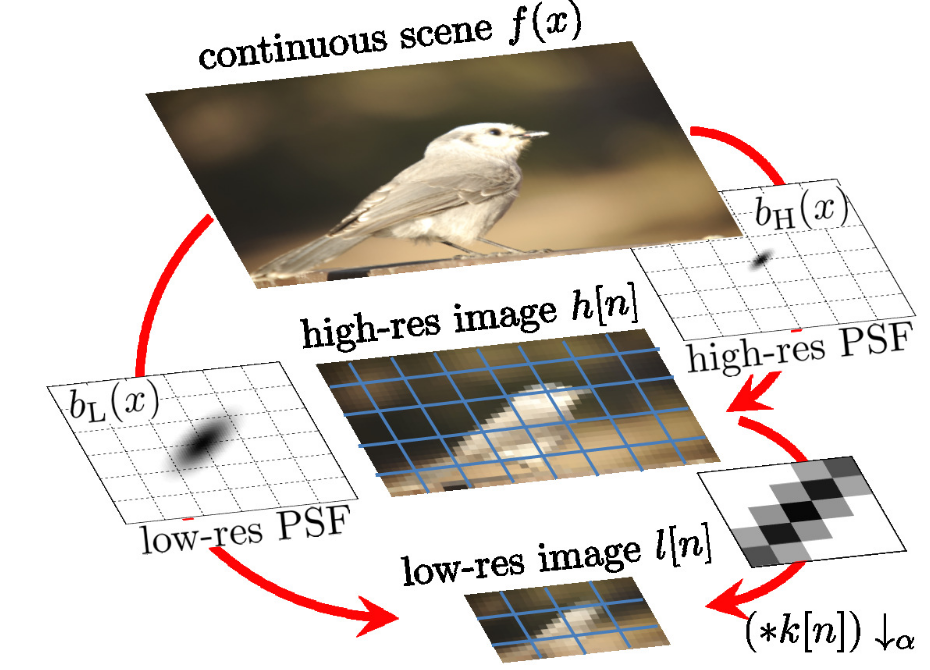
\includegraphics[width=0.5\textwidth]{RelationBtwImages.png}
	\caption{}
	\label{fig:RelationBtwImages}
\end{figure}
In Figure \ref{fig:1DBlur} a one-dimensional visual representation of a naive and a more optimal blur kernel can be seen. The naive blur kernel $k_{\text{naive}}$ is a discretization of the one-dimensional rectangular PSF $b_L(x)$, and the optimal blur kernel $k_{\text{optimal}}$ may look very different from this - even with negative values and a more oscillatory nature.
\begin{figure}
	\centering
	\begin{subfigure}[b]{0.4\textwidth}
		\centering
		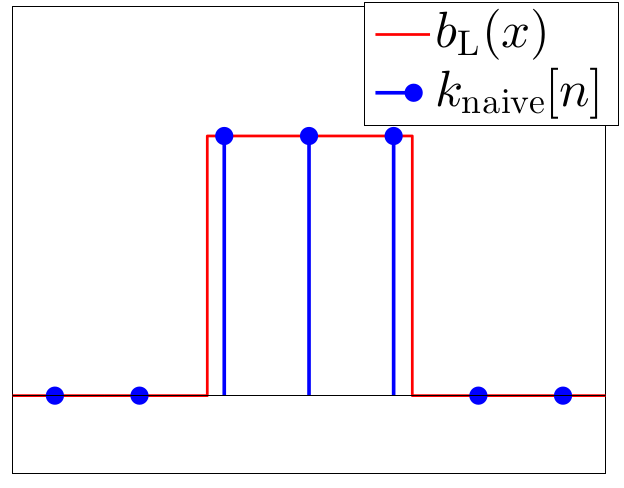
\includegraphics[width=\textwidth]{1DBlurNaive.png}
		\caption{}
		\label{fig:1DBlurNaive}
	\end{subfigure}
	~
	\begin{subfigure}[b]{0.42\textwidth}
		\centering
		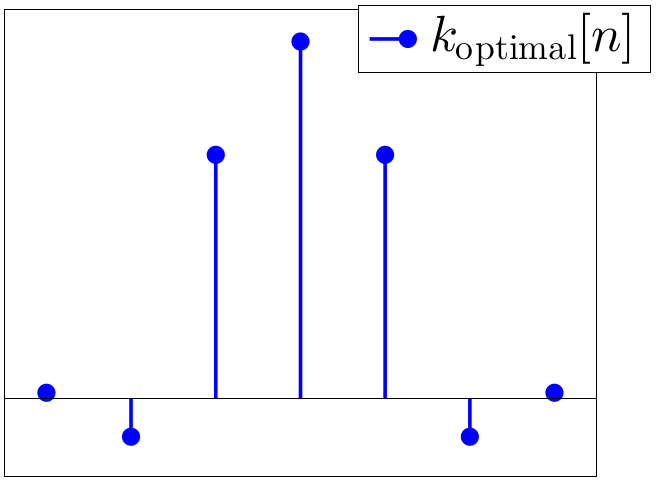
\includegraphics[width=\textwidth]{1DBlurComputed.png}
		\caption{}
		\label{fig:1DBlurComputed}
	\end{subfigure}
	\caption{$k_{\text{naive}}[n]$ is a discretization of the low-resolution PSF $b_L(x)$, (\ref{fig:1DBlurNaive}), but the actual optimal blur kernel $k_{\text{optimal}}[n]$ may be very different, (\ref{fig:1DBlurComputed}).}
	\label{fig:1DBlur}
\end{figure}

The actual blur kernel $k$ is composed of two operations. A deconvolution with the high-resolution PSF $b_H(x)$ followed by a convolution with the low-resolution PSF $b_L$. $k$ should thus have the same effect as a continuous-domain filter $k_c$, whose Fourier transform is:
\begin{equation}
	K_c(\omega) = \frac{B_L(\omega)}{B_H(\omega)} = \frac{B_L(\omega)}{B_L(\frac{\omega}{\alpha})}
	\label{eq:ContKFourierTrans}
\end{equation}


\begin{figure}[h]
	\centering
	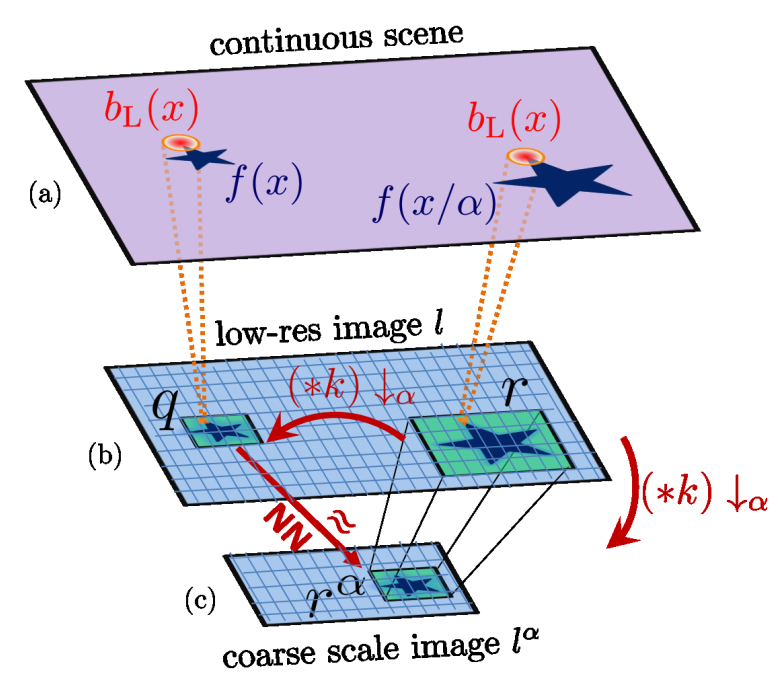
\includegraphics[width=0.5\textwidth]{PatchRecurrenceVis.png}
	\caption{}
	\label{fig:PatchRecurrenceVisual}
\end{figure}
	\begin{appendices}
	\end{appendices}
	
\end{document}